\taskpic{
	Модель водяного колеса устроена следующим образом: на ободе колеса радиусом $R = 1 \unit{м}$
    равномерно расположены $N$ ячеек, причём $N = 201$. Когда очередная ячейка проходит верхнее
    положение, в неё сбрасывается (без начальной скорости относительно земли) груз массой $m = 100
    \unit{г}$. Когда ячейка проходит нижнее положение, груз вываливается из неё без начальной скорости
    относительно колеса. Масса самого колеса мала, все удары абсолютно неупругие, трения нет. Найдите
    установившуюся угловую скорость вращения колеса.
}{
	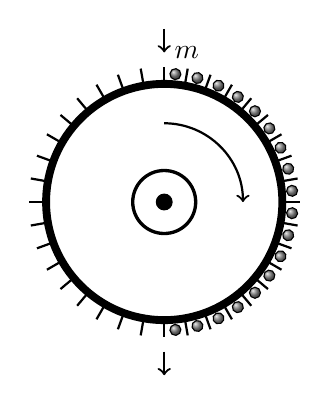
\begin{tikzpicture}
    	\draw[line width = 0.1cm] (0, 0) circle (1.5cm);
        \draw[very thick] (0, 0) circle (0.4cm);
        \draw[fill = black] (0, 0) circle (0.1cm);
        \draw[thick, ->] (0, 1cm) arc (90:0:1cm);
        \foreach \x in {0, 10, 20, ..., 360}{
        	\draw[thick, rotate around = {\x:(0, 0)}] (0, 1.5) -- ++(0, 0.22cm);
        }
        \foreach \y in {5, 15, 25, ..., 175}{
        	\draw[ball color = gray, rotate around = {-\y:(0, 0)}] (0, 1.63cm) circle (0.07cm);
        }
        \draw[thick, ->] (0, 2.2) -- ++(0, -0.3cm) node[right] {$m$};
        \draw[thick, ->] (0, -1.9) -- ++(0, -0.3cm);
  \end{tikzpicture}
}
% Москва, город-1996, 11 класс